\chapter{Storage Layout \& Management}
\label{ch:MM}
\section{Layout and run-time organization}
A crucial property of the Oberon is centralized resource management. Its advantage is that
replication of management algorithms and a premature partitioning of resources are avoided. The
disadvantage is that management algorithms are fixed once and forever and remain the same for
all applications. The success of a centralized resource management therefore depends crucially on
its flexibility and its efficient implementation. This chapter presents the scheme and the algorithms
governing main storage in the Oberon.

The storage layout of the Oberon is determined by the structure of code and data typical in
the use of modular, high-level programming languages, and in particular of the language Oberon. It
suggests the subdivision of storage into three areas.
\begin{enumerate}
	\item The module space. Every module specifies procedures (code) and global (static) variables. Its
initialization part can be regarded as a procedure implicitly called after loading. Upon loading, space
must be allocated for code and data. Typically, modules contain very few or no global variables,
hence the size of the allocated space is primarily determined by the code. The combined code and
data space is called a block. Blocks are allocated in the module space by the loader.
	\item The workspace (stack). Execution of every command invokes a sequence of procedures, each of
which uses (possibly zero) parameters and local variables. Since procedure calls and completions
follow a strict first-in last-out order, the stack is the uniquely suited strategy for storage allocation for
local data. Deallocation upon completion of a procedure is achieved by merely resetting the pointer
identifying the top of the stack. Since this operation is performed by a single instruction, it costs
virtually no time. Because Oberon is a single-process system, a single stack suffices. Furthermore,
after completion of a command, the stack is empty. This fact will be important in simplifying the
scheme for reclamation of dynamically allocated space.
	\item The dynamic space (heap). Apart from global (static) variables, and local (stack-allocated)
variables, a program may refer to anonymous variables referenced through pointers. Such
variables are allocated truly dynamically through calls of an explicit operation (NEW). These
variables are allocated in the so-called heap. Their deallocation is "automatic", when free storage is
needed and they are no longer referenced from any of the loaded modules. This process is called
garbage collection. Every record allocated in the heap contains a (hidden) pointer to the descriptor
of its type called the type tag. It is used by the garbage collector.
\end{enumerate}

Unfortunately, the number of distinct spaces is larger than two. If it were two, no arbitrary size
limitation would be necessary; merely the sum of their sizes would be inherently limited by the size
of the store. In the case of three spaces, arbitrarily determined size limits are unavoidable. Addressmapping hardware can alleviate (and delegate) this problem using a virtual address space which is
so large that limits will hardly ever be reached.

Such a scheme is implemented by tables mapping virtual into physical addresses, requiring multiple
memory accesses for every reference. Of course, the need for a double or a triple access for every
memory reference is avoided by a translation cache in the (hardware) unit. Nevertheless, a
decrease in performance is unavoidable for each cache miss. Furthermore, an additional subcycle
is required for every access in order to look up the cached translation table. Without a virtual
address scheme, each module block must consist of an integral number of physically adjacent
pages. Holes generated by the release of modules must be reused. We employ the simple scheme
of marking the released space as a hole, and of allocating a new block in the first hole encountered
that is large enough (first-fit strategy). Considering the relative infrequency of module releases,
efforts to improve the strategy are not worth the resulting added complexity.

It is remarkable that the code for module allocation and release without virtual addressing is only
marginally more complicated than with it. The only remaining advantages of an MMU are a better
storage utilization, because no holes occur (a negligible advantage), and that inadvertent
references to unloaded modules, e.g. via installed procedures, lead to an invalid address trap.

It is worth recalling that the concept of address mapping was introduced as a requirement for virtual
memory implemented with disks as backing store, where pages could be moved into the
background in order to obtain space for newly required pages, and could then be retrieved from
disk on demand, i.e. when access was requested. This scheme is called demand paging. It is not
used in the Oberon, and one may fairly state that demand paging has lost its significance
with the availability of large, primary stores.

Experience in the use of the RISC predecessor Ceres leads to the conclusion that whereas address
translation through an MMU was an essential feature for multi-user OSes, it constitutes
a dispensible overkill for single-user workstations. The fact that modern semiconductor technology
made it possible to integrate the entire translation and caching scheme into a single chip, or even
into the processor itself, led to the hiding (and ignoring) of the scheme's considerable complexity.
Its side effects on execution speed are essentially unpredictable. This makes systems with MMU
virtually unusable for applications with tight real-time constraints. The RISC processor does indeed
not feature an address mapping unit.

The RISC processor features 16 registers (of 32 bits). R0 - R11 are used for expression evaluation.
R12 - R15 have fixed, system-wide usage:
\begin{table}[h!]
	\centering
	\begin{tabular}{l l}
		R12 & address of the module table MT (typically constant) \\
		R13 & base address for variables in the current module SB (static base) \\
		R14 & stack pointer SP \\
		R15 & return address LNK (fixed by RISC's BL instruction)
	\end{tabular}
\end{table}

The used memory layout is shown in Figure 8.1.
\begin{figure}
	\label{fig:storage-layout}
	\centering
	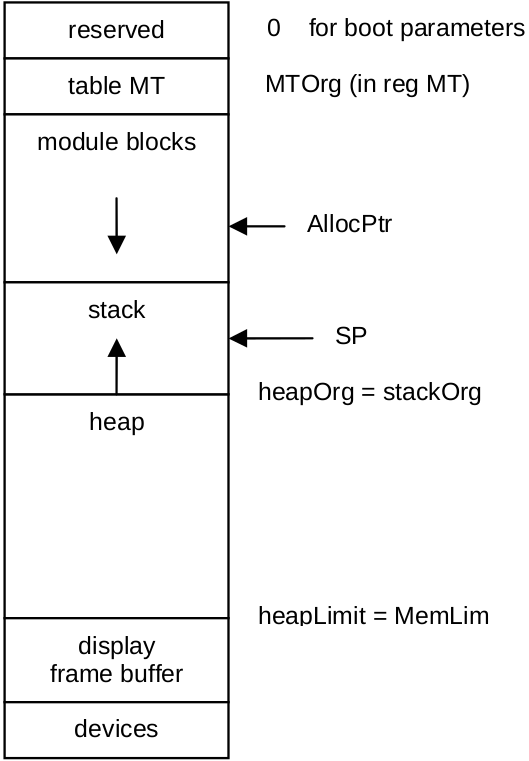
\includegraphics[width=.5\textwidth]{i/q}
	\caption{Storage layout}
\end{figure}

\section{Management of dynamic storage}
The term dynamic storage is used here for all variables that are allocated neither statically (global
variables) nor on the stack (local variables), but through invocation of the intrinsic procedure NEW.
Such variables are anonymous and are referenced exclusively via pointers. The space in which
they are allocated is called the heap.

The space allocated to such dynamic variables becomes free and reusable as soon as the last
reference to it vanishes. This event is hard, and in multiprocess systems even impossible to detect.
The usual remedy is to ignore it and instead to determine the accessibility of all allocated variables
(records, objects) only at the time when more storage space is needed. This process is then called
garbage collection.

The Oberon does not provide an explicit deallocation procedure allowing the programmer
to signal that a variable will no longer be referenced. The first reason for this omission is that
usually a programmer would not know when to call for deallocation. And secondly, this "hint" could
not be taken as trustworthy. An erroneous deallocation, i.e. one occurring when there still exist
references to the object in question, could lead to a multiple allocation of the same space with
disastrous consequences. Hence, it appears wise to fully rely on system management to determine
which areas of the store are truly reusable.

Before discussing the scheme for storage reclamation, which is the primary subject of dynamic
storage management, we turn our attention to the problem of allocation, i.e. the implementation of
procedure NEW. The simplest solution is to maintain a list of free blocks and to pick the first one
large enough. This strategy leads to a relatively large fragmentation of space and produces many
small elements, particularly in the first part of the list. We therefore employ a somewhat more
refined scheme and maintain four lists of available space. Three of them contain pieces of fixed
size, namely 32, 64, and 128 bytes. The fourth list contains pieces whose size is any multiple of
256. We note that the choice of the values permits the merging of any two contiguous elements into
an element of the next list. This scheme keeps fragmentation, i.e. the emergence of small pieces in
large numbers, reasonably low with minimal effort. The body of procedure NEW consists of
relatively few instructions, and typically only a small fraction of them needs to be executed.

The statement NEW(p) is compiled into an instruction sequence assigning the address of pointer
variable p to a fixed register (R0) and the type tag to another register (R1). The type tag is a pointer
to a type descriptor containing information required by the garbage collector. This includes the size
of the space occupied and now to be allocated. The effect of NEW is the assignment of the address
of the allocated block to p, and the assignment of the tag to a prefix of the block. (see Fig. 8.2)
\begin{figure}
	\label{fig:allocation}
	\centering
	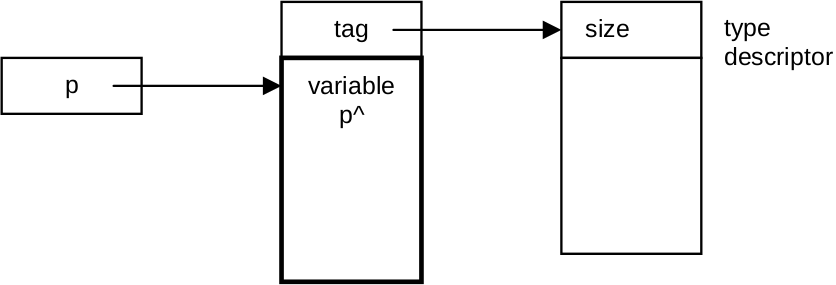
\includegraphics[width=\textwidth]{i/r}
	\caption{Allocation of dynamic variable $\hat{p}$ in the heap by procedure $NEW(p)$}
\end{figure}
In conclusion, we emphasize that this scheme makes the allocation of an object very efficient.
Nevertheless, it is considerably more costly than that of a variable explicitly declared and therefore
allocated either globally or on the stack.
We now turn to the problem of storage reclamation or garbage collection. There exist two
essentially different schemes: the reference counting and the mark-scan schemes. In the former,
every object carries a (hidden) reference count, indicating the number of existing references to it.
The scheme works as follows:
1. NEW(p) initializes the reference count of $\hat{p}$ to 1.
2. An assignment q := p decrements the reference count of $\hat{q}$ by 1, performs the assignment,
then increments the reference count of $\hat{p}$ by 1. When a reference count reaches zero, the
element is linked into the free list.

There are two disadvantages inherent in this approach. The first is the non-negligible overhead in
pointer assignments. The second is that circular data structures never become recognized as free,
even if no external references point to their elements.

The Oberon employs the second scheme which involves no hidden operations like the
reference counting scheme, but relies on a process initiated when free storage has become scarce
and more is needed. It consists of two phases. In the first phase, all referenced and therefore still
accessible elements are marked. In the second phase, their unmarked complement is released.

The first phase is called the mark phase, the second the scan phase. Its primary disadvantage is
that the process may be started at moments unpredictable to the system's user. During the
process, the computer then appears to be blocked. It follows that an interactive system using markscan garbage collection must guarantee that the process is sufficiently fast in order to be hardly
noticeable. Modern processors make this possible, even with large main stores. Nevertheless,
finding all accessible nodes in an entire computer system within, say, a second appears to be a
formidable feat.

We recognize that the mark phase essentially is a tree traversal, or rather a forest traversal. The
roots of the trees are all named pointer variables in existence. We shall postpone the question of
how these roots are to be found, and first present a quick tutorial about tree traversal. In general,
nodes of the traversed structure may contain many pointers (branches). We shall, however, first
restrict our attention to a binary tree, because the essential problem and its solution can be
explained better in this way.

The essential problem alluded to is that of storage utilization by the traversal algorithm itself.
Typically, information about the nodes already visited must be retained, be it explicitly, or implicitly
as in the case of use of recursion. Such a strategy is plainly unacceptable, because the amount of
storage needed is unpredictable and may become very large, and because garbage collection is
typically initiated just when more storage is unavailable. The task may seem impossible, yet a
solution lies in the idea of inverting pointers along the path traversed, thus keeping the return path
open. It is embodied in the following procedure, whose task is to traverse the tree given by the
parameter root, and to mark every node. Mark values are assumed to be initially 0. Let the data
structure be defined by the types
\begin{verbatim}
Ptr = POINTER TO Node;
Node = RECORD m: INT; L, R: Ptr END;
\end{verbatim}
and the algorithm by the procedure
\begin{verbatim}
PROC traverse(root: Ptr);
VAR p, q, r; Ptr;
BEGIN p := root; q := root;
REPEAT (* p # NIL *) INC(p.m); (*mark*)
IF p.L # NIL THEN (*pointer rotation*)
r := p.L; p.L := p.R; p.R := q; q := p; p := r
ELSE
p.L := p.R; p.R := q; q:= NIL
END
UNTIL p = q
END traverse
\end{verbatim}

We note that only three local variables are required, independent of the size of the tree to be
traversed. The third, r, is in fact merely an auxiliary variable to perform the rotation of values p.L,
p.R, q, and p as shown in Fig. \ref{fig:rotation}. A snapshot of a tree traversal is shown in Fig. \ref{fig:tree-traversal}.
\begin{figure}
	\label{fig:rotation}
	\centering
	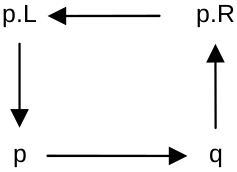
\includegraphics[width=.25\textwidth]{i/s}
	\caption{Rotation of four pointers}
\end{figure}
\begin{figure}
	\label{fig:tree-traversal}
	\centering
	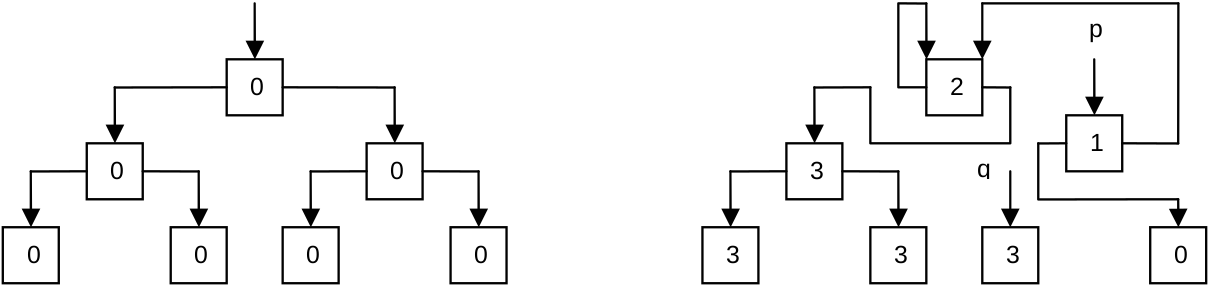
\includegraphics[width=\textwidth]{i/t}
	\caption{Tree traversal (original at left, snapshot at right)}
\end{figure}
The pair p, q of pointers marks the position of the process. The algorithm traverses the tree in a left
to right, depth first fashion. When it returns to the root, all nodes have been marked.
How are these claims convincingly supported? The best way is by analyzing the algorithm at an
arbitrary node. We start with the hypothesis H that, given the initial state P, the algorithm will reach
state Q, (see Fig \ref{fig:transition}).
State Q differs from P by the node and its descendants B and C having been marked, and by an
exchange of p and q. We now apply the algorithm to state P, assuming that B and C are not empty.
The process is illustrated in Fig \ref{fig:transition}. P0 stands for P in Fig. \ref{fig:tree-traversal}.
\begin{figure}
	\label{fig:transition}
	\centering
	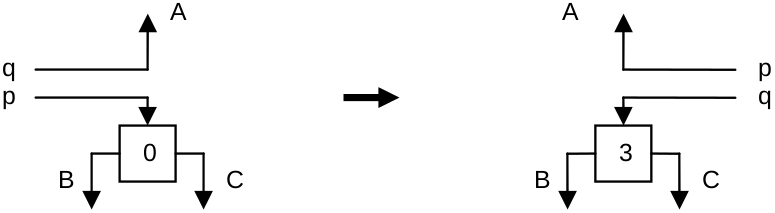
\includegraphics[width=\textwidth]{i/u}
	\caption{Transition from state P to Q}
\end{figure}

Transitions $P0 \rightarrow P1$, $P2 \rightarrow P3$, and $P4 \rightarrow P5$ are the direct results of applying the pointer rotation
as specified by the sequence of five assignments in the algorithm. Transitions $P1 \rightarrow P2$ and $P3 \rightarrow P4$ follow from the hypothesis H being applied to the states P1 and P3: subtrees are marked and p,
q interchanged. We note in passing that the node is visited three times. Progress is recorded by the
mark value which is incremented from 0 to 3.

Fig. \ref{fig:transition-3-times}. demonstrates that, if H holds for steps $P1 \rightarrow P2$ and $P3 \rightarrow P4$, then it also holds for step
$P1 \rightarrow P5$, which visits the subtree p. Hence, it also holds for the step root $\rightarrow$ root, which traverses
the entire tree.
\begin{figure}
	\label{fig:transition-3-times}
	\centering
	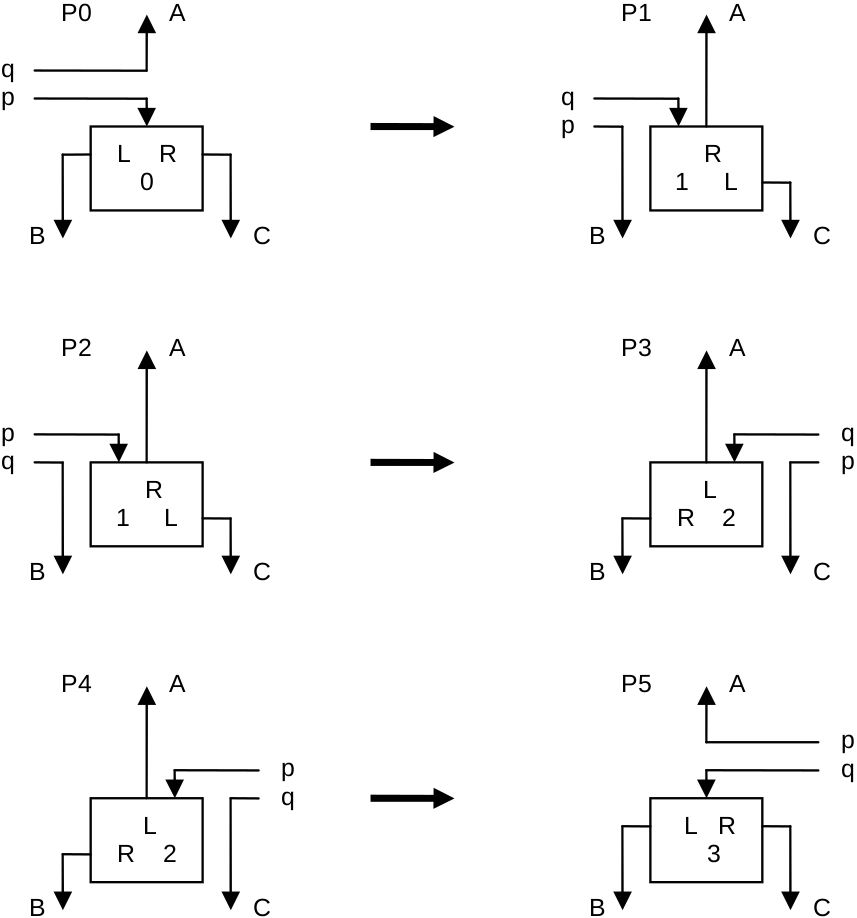
\includegraphics[width=.9\textwidth]{i/v}
	\caption{Transitions from P0 to P5, visiting nodes 3 times}
\end{figure}

This proof by recursion relies on the algorithm performing correct transitions also in the case of p.L
being NIL, i.e. B being the empty tree. In this case, state P1 is skipped; the first transition is $P0 \rightarrow P2$ (see Fig \ref{fig:transition-direct}).
If p.L is again NIL, i.e. also C is empty, the next transition is $P2 \rightarrow P4$. This concludes the
demonstration of the algorithm's correctness.
\begin{figure}
	\label{fig:transition-direct}
	\centering
	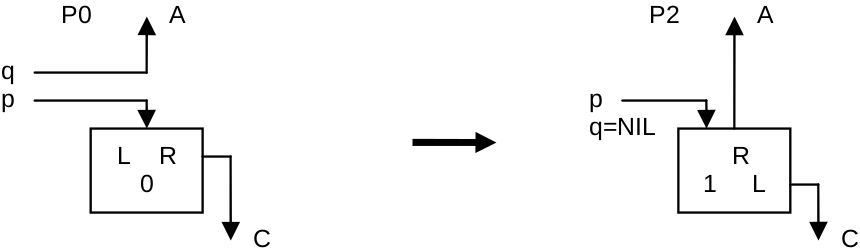
\includegraphics[width=\textwidth]{i/w}
	\caption{Direct transition from P0 to P2, if $p.L = NIL$}
\end{figure}

We now modify the algorithm of tree traversal to the case where the structure is not confined to a
binary tree, but may be a tree of any degree, i.e. each node may have any number n of
descendants. For practical purposes, however, we restrict n to be in the range $0 \leq n \leq N$, and
therefore may represent all nodes by the type
\begin{verbatim}
Node = RECORD m, n: INT;
dsc: ARRAY N OF Node
END
\end{verbatim}

In principle, the binary tree traversal algorithm might be adopted almost without change, merely
extending the rotation of pointers from p.L, p.R, q, p to p.dsc[0], ... , p.dsc[n-1], q, p. However, this
would be an unnecessarily inefficient solution. The following is a more effective variant. Moreover, it
caters for the case of inhomogeneous graphs, where different nodes have different numbers of
descendants. The key lies in associating with every node, in addition to the tag, a second private
field mk. It serves two purposes. The first is as a mark, with mk > 0 indicating that the node had
been visited. The second is to store the address of the next descendant to be visited. The
underlying data structure is shown in Fig \ref{fig:record}. Type descriptors consist of the following fields:
\begin{table}[h!]
	\centering
	\setlength{\tabcolsep}{2pt}
	\begin{tabular}{l l}
		size & {\small in bytes, of the described record type,} \\
		base & {\small a table of pointers to the base types descriptors(3 elements only)} \\
		{\small offsets} & {\small of the descendant pointers in the described type(1 word each)}
	\end{tabular}
\end{table}
\begin{figure}
	\label{fig:record}
	\centering
	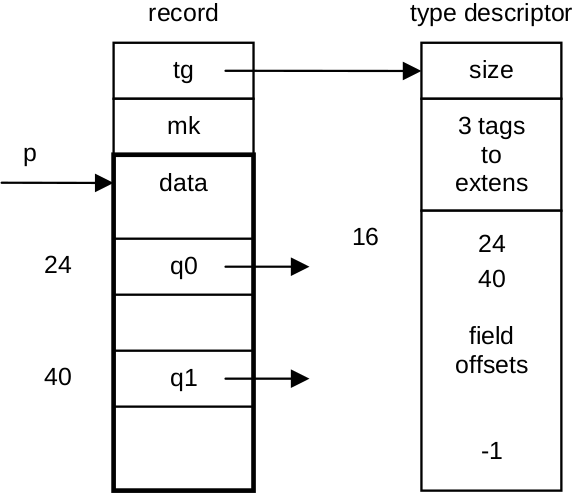
\includegraphics[width=.9\textwidth]{i/x}
	\caption{Record and its type descriptor}
\end{figure}

We note that the mark value, starting with zero (unmarked), is used as a counter of descendants
already traversed, and hence as an index to the descendant field to be processed next. The
algorithm can be applied not only to trees, but to arbitrary structures, including circular ones, if the
continuation condition p \# 0 (actually p >= heapOrg) is extended to (p >= heapOrg) \& (offadr = 0).
This causes a descendant that is already marked to be skipped. Here the array M stands for the
entire memory.
\begin{verbatim}
PROC traverse(root: Ptr);
VAR offadr, offset: INT; p, q, r: Ptr;
BEGIN p := root; q := root;
REPEAT (* p # NIL*) offadr := p.mk; (*mark*)
IF offadr = 0 THEN tag := p.tg; offadr := tag + 16 ELSE INC(offadr, 4) END ;
p. mk := offadr; offset := M[offadr];
IF offset # -1 THEN (*move down*)
r := M[p+offset]; offadr := M[r-4];;
IF offadr = 0 THEN M[p+offset] := q; q := p; p := r END
ELSE (*move up*)
offadr := M[q-4];offset := M[offadr]
IF p # q THEN r := M[q+offset]; M[q+offset] := p; p := q; q := r END
END
UNTIL (p = q) & (offset = -1)
END traverse;
\end{verbatim}

The mark is included in each record's hidden prefix. The prefix takes 2 words only; the first is used
for the tag. The other is reserved for the garbage collector and used as mark and offset address.
The end of the list of descendant pointers is marked by an entry with value -1. And finally,
assignments involving M are expressed as
\begin{table}[h!]
	\centering
	\begin{tabular}{c c c}
		$SYSTEM.GET(a, x)$ & for & $x := M[a]$ \\
		$SYSTEM.PUT(a, x)$ & for & $M[a] := x$ \\
	\end{tabular}
\end{table}

The scan phase is performed by a relatively straight-forward algorithm. The heap, i.e. the storage
area between HeapOrg and HeapLimit (the latter is a variable), is scanned element by element,
starting at HeapOrg. Elements marked are unmarked, and unmarked elements are freed by linking
them into the appropriate list of available space.
As the heap may always contain free elements, the scan phase must be able to recognize them in
order to skip them or merge them with an adjacent free element. For this purpose, the free
elements are also considered as prefixed. The prefix serves to determine the element's size and to
recognize it as free due to a special (negative) mark value. The encountered mark values and the
action to be taken are:
\begin{table}[h!]
	\centering
	\begin{tabular}{c r c}
		mk value &  state   & action \\\hline
		$=0$     & unmarked & collect, mark free \\
		$>0$     &   marked & unmark \\
		$<0$     &     free & skip or merge
	\end{tabular}
\end{table}

\section{Kernel}
The kernel lies at the bottom of the module hierarchy. It contains the procedures for dynamic
storage allocation and retrieval as described before. The procedures are New, Mark, and Scan.
Kernel also contains the driver routines for the disk. They are used by modules FileDir and Files.
The "disk" is actually an SD-card, a high-volume flash-RAM. It is accessed purely sequentially,
byte-wise, by a standard, serial peripheral interface (SPI). Within Kernel a table called SectorMap is
allocated keeping track of blocks (sectors) occupied by files. A single bit indicates, whether a sector
is allocated or not. This table is accessed by the procedures AllocSector, MarkSector, and
FreeSector. Reading and writing is done sector-wise by procedures GetSector and PutSector.
Sector numbers are always a multiple of 29 for the purpose of redundancy checks.

Furthermore, the kernel contains a timer counting milliseconds and, perhaps, a real time clock,
showing date and time. Clock data are packed into a single word as follows:
\begin{figure}
	\label{fig:datetime}
	\centering
	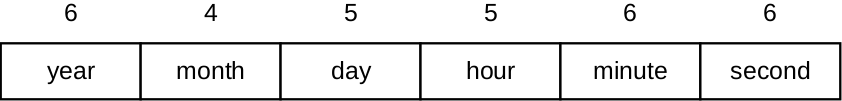
\includegraphics[width=\textwidth]{i/y}
	\caption{Encoding of date and time (year starting with 2000)}
\end{figure}
\begin{verbatim}
DEFINITION Kernel; (*NW/PR 11.4.86 / 27.12.95 / 15.5.2013*)
CONST SectorLength = 1024;
TYPE Sector = ARRAY SectorLength OF BYTE;
VAR allocated, NofSectors: INT;
heapOrg, heapLim: INT;
stackOrg, MemSize: INT;
PROC New(VAR ptr: INT; tag: INT);
PROC Mark(pref: INT);
PROC Scan;
PROC ResetDisk;
PROC MarkSector(sec: INT);
PROC FreeSector(sec: INT);
PROC AllocSector(hint: INT; VAR sec: INT);
PROC GetSector(src: INT; VAR dest: Sector);
PROC PutSector(dest: INT; VAR src: Sector);
PROC Time(): INT; (*milliseconds*)
PROC Clock(): INT;
PROC SetClock(dt: INT);
PROC Install(adr, procadr: INT);
PROC Init;
END Kernel.
\end{verbatim}

\section{The storage management's toolbox}
The user can obtain information about the system's state and resources through its toolbox, a set of
commands contained in the too module System. These commands are:
\begin{verbatim}
PROC Watch;
PROC Collect; / n
PROC SetClock; / year, month, day, hour, minute, second
\end{verbatim}

Command Watch shows the amount of storage occupied in the heap, the number of disk sectors
allocated on the disk, and the number of tasks installed. The command Collect allows to control the
frequency of garbage collections. The number n indicates how many commands are executed
before the next garbage collection.
